\begin{frame}{Activité: Le crêpier psycho-rigide}

  \begin{block}{Matériel}
    \begin{itemize}
    \item des planchettes en bois de tailles et de couleurs différentes (faces reconnaissables)
    \item éventuellement une pelle à tarte pour retourner les planchettes
    \end{itemize}
  \end{block}

  \begin{block}{Règle du jeu}
    \begin{itemize}
      \item \structure{Installation :} Faire une pile désordonnée de crêpes.
      \item \structure{Objectif :} ranger les crêpes de la plus grande (en bas) à la plus petite (au haut), face colorée vers le haut.
      \item \structure{Coup autorisé :} prendre une ou plusieurs crêpes sur le haut de la pile, et de les reposer à l'envers.
    \end{itemize}
  \end{block}

  \bigskip \bigskip \bigskip

  \begin{center}
    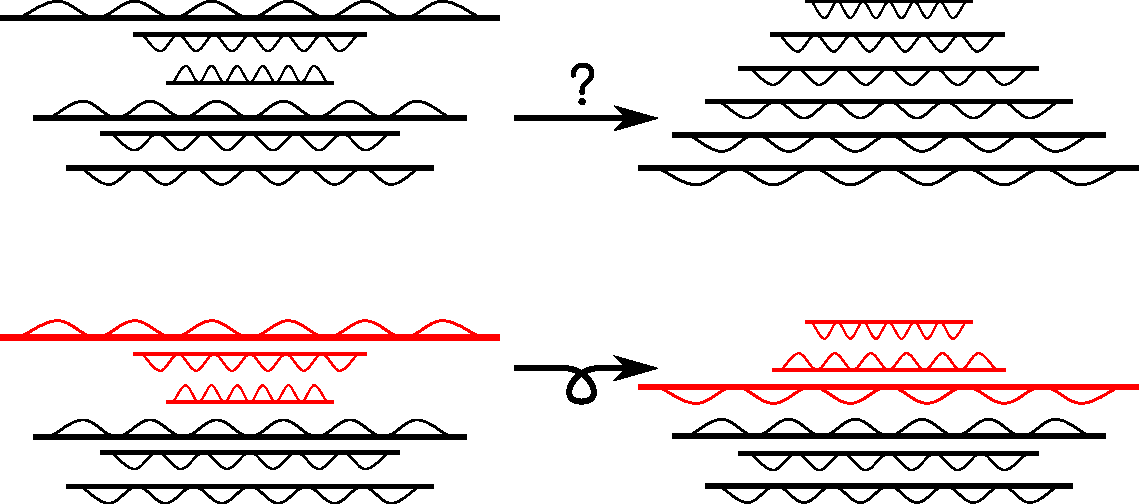
\includegraphics[width=0.8\linewidth]{img/crepier.pdf}
  \end{center}

\end{frame}

\begin{frame}{Ce qu'il faut retenir du  crêpier psycho-rigide}

  \begin{columns}
    \begin{column}{.7\linewidth}
      \begin{block}{Un algorithme}
        \begin{itemize}
        \item n'a d'intérêt que si on peut l'expliquer
        \item doit être suffisamment simple pour pouvoir l'expliquer à une machine
        \item \alert{\textbf{«Diviser pour mieux régner»}} : on essaie toujours de décomposer un algorithme en tâches simples
        \end{itemize}
      \end{block}

      \begin{block}{L'algorithme que doit suivre le crêpier est :}
        \begin{itemize}
        \item ramener la plus grande crêpe en haut de la pile
        \item retourner pour que la face brûlée soit vers le haut
        \item retourner la pile de sorte à mettre la plus grande crêpe en bas
        \item réitérer avec la crêpe de taille inférieure
        \end{itemize}
      \end{block}

      \begin{block}{Le rapport avec l'informatique}
        \begin{itemize}
        \item l'informaticien passe son temps à trouver des algorithmes et  à les expliquer à la machine
        \item le principe \alert{\textbf{«Diviser pour mieux régner»}} est fondamental en informatique
        \end{itemize}
      \end{block}
    \end{column}

    \begin{column}{.3\linewidth}
      \begin{block}{Pour aller plus loin}
        Selon l'état initial de la pile de crêpes, le nombre minimum de coups nécessaires pour la ranger varie.

        \begin{itemize}
          \item Quel est le meilleur état initial possible (qui demandera le moins de coups pour ranger) ?
          \item Quel est le pire état initial possible ?
          \item Combien faut-il de coups pour ranger une pile de $N$ crêpes dans le pire des cas ?
        \end{itemize}
      \end{block}
    \end{column}
  \end{columns}
      
\end{frame}

\begin{frame}{Ce qu'il faut retenir du crêpier psycho-rigide : performance d'algorithmes}

  \begin{block}{Pourquoi évaluer la performance d'un algorithme ?}

    Évaluer la performance d'un algorithme nous permet :

    \begin{itemize}
      \item de se faire une idée du temps nécessaire pour résoudre un problème de plus grande taille (combien de temps pour un million de crêpes ?) ;
      \item de le comparer à d'autres aglorithmes résolvant le même problème, pour savoir lequel est le meilleur.
    \end{itemize}

  \end{block}

  \begin{block}{Comment évaluer la performance d'un algorithme ?}

    \begin{itemize}
      \item On compte le nombre de coups nécessaires dans le cas général. Pour le crêpier :
        \begin{itemize}
          \item pour ranger une crêpe, il faut entre $0$ coups (la crêpe est déjà rangée) et $3$ coups (amener en haut, retourner, amener à sa place) ;
          \item pour $n$ crêpes (cas général), il faut entre $0$ et $3 \times n$ coups ;
          \item la performance d'un algorithme sur un cas particulier dépend donc beaucoup de l'état initial, mais en règle générale on s'intéresse surtout aux cas intermédiaires, qui sont les plus probables.
        \end{itemize}
      \item $n$ est une variable qui exprime la taille du problème. La performance d'un algorithme est notée comme une fonction de la taille du problème nommée $O$.
      \item La performance exprime un ordre de grandeur plutôt qu'une évaluation précise du temps d'exécution. Pour des grandes valeurs de $n$, il n'est pas très utile de faire la distinction entre $O(n)$, $O(n+4)$ ou encore $O(3 \times n)$ - surtout quand on compare avec un autre algorithme dont la performance est $O(n^2)$. 
      \item On simplifie donc en retirant les constantes pour ne garder que les termes les plus importants. Pour le crêpier, on notera la performance de notre algorithme $O(n)$ ; on dit alors que le temps de calcul croit \textit{linéairement} avec $n$. En revanche, un algorithme $O(n^2)$ aurait une croissance \textit{quadratique}, et un algorithme $O(2^n)$ aurait une croissance \textit{exponentielle}.
     \end{itemize}
  \end{block}

  \begin{block}{À la recherche du meilleur algorithme possible}
    \begin{itemize}
    \item On arrive parfois à montrer qu'on a le meilleur algorithme possible. Par exemple on ne peut pas trier les éléments en moins de $n$ étapes, car on doit forcément tous les considérer.
    \item On peut aussi prouver qu'un tri comparatif ne peut pas se faire en moins de $n\times log(n)$ étapes, car il n'accumule pas assez d'information pour choisir la bonne permutation en moins d'étapes.
    \item Mais la plupart du temps, on ne sait pas prouver que l'algorithme connu est le meilleur possible. C'est alors le meilleur \textit{connu}, sans être forcément le meilleur \textit{possible}.
    \end{itemize}
  \end{block}

  %\begin{block}{À la recherche de problèmes difficiles}
    %\begin{itemize}
    %\item On peut classifier les problèmes en fonction de la performance des algorithmes les résolvant. \\
      %(cela permet de se forger un sens commun de ce qui est faisable avec un ordinateur et éviter les problèmes si difficiles qu'ils sont quasi impossibles)
    %\item Il existe énormément de problèmes relativement simples pour lesquels personne ne connaît de bon algorithme, sans que personne n'arrive non plus à démontrer qu'un tel algorithme n'existe pas.
    %\item L'activité suivante sera l'occasion d'explorer un peu cette classification des problèmes très durs.
    %\end{itemize}
  %\end{block}
\end{frame}
